% P5 -- AUROC degradation
\begin{frame}[t]{AUROC degradation: the one genuinely new phenomenon}{The confidence \emph{ranking} decays when evidence is genuinely evicted}
  \begin{columns}[T]
    \begin{column}{0.44\textwidth}
      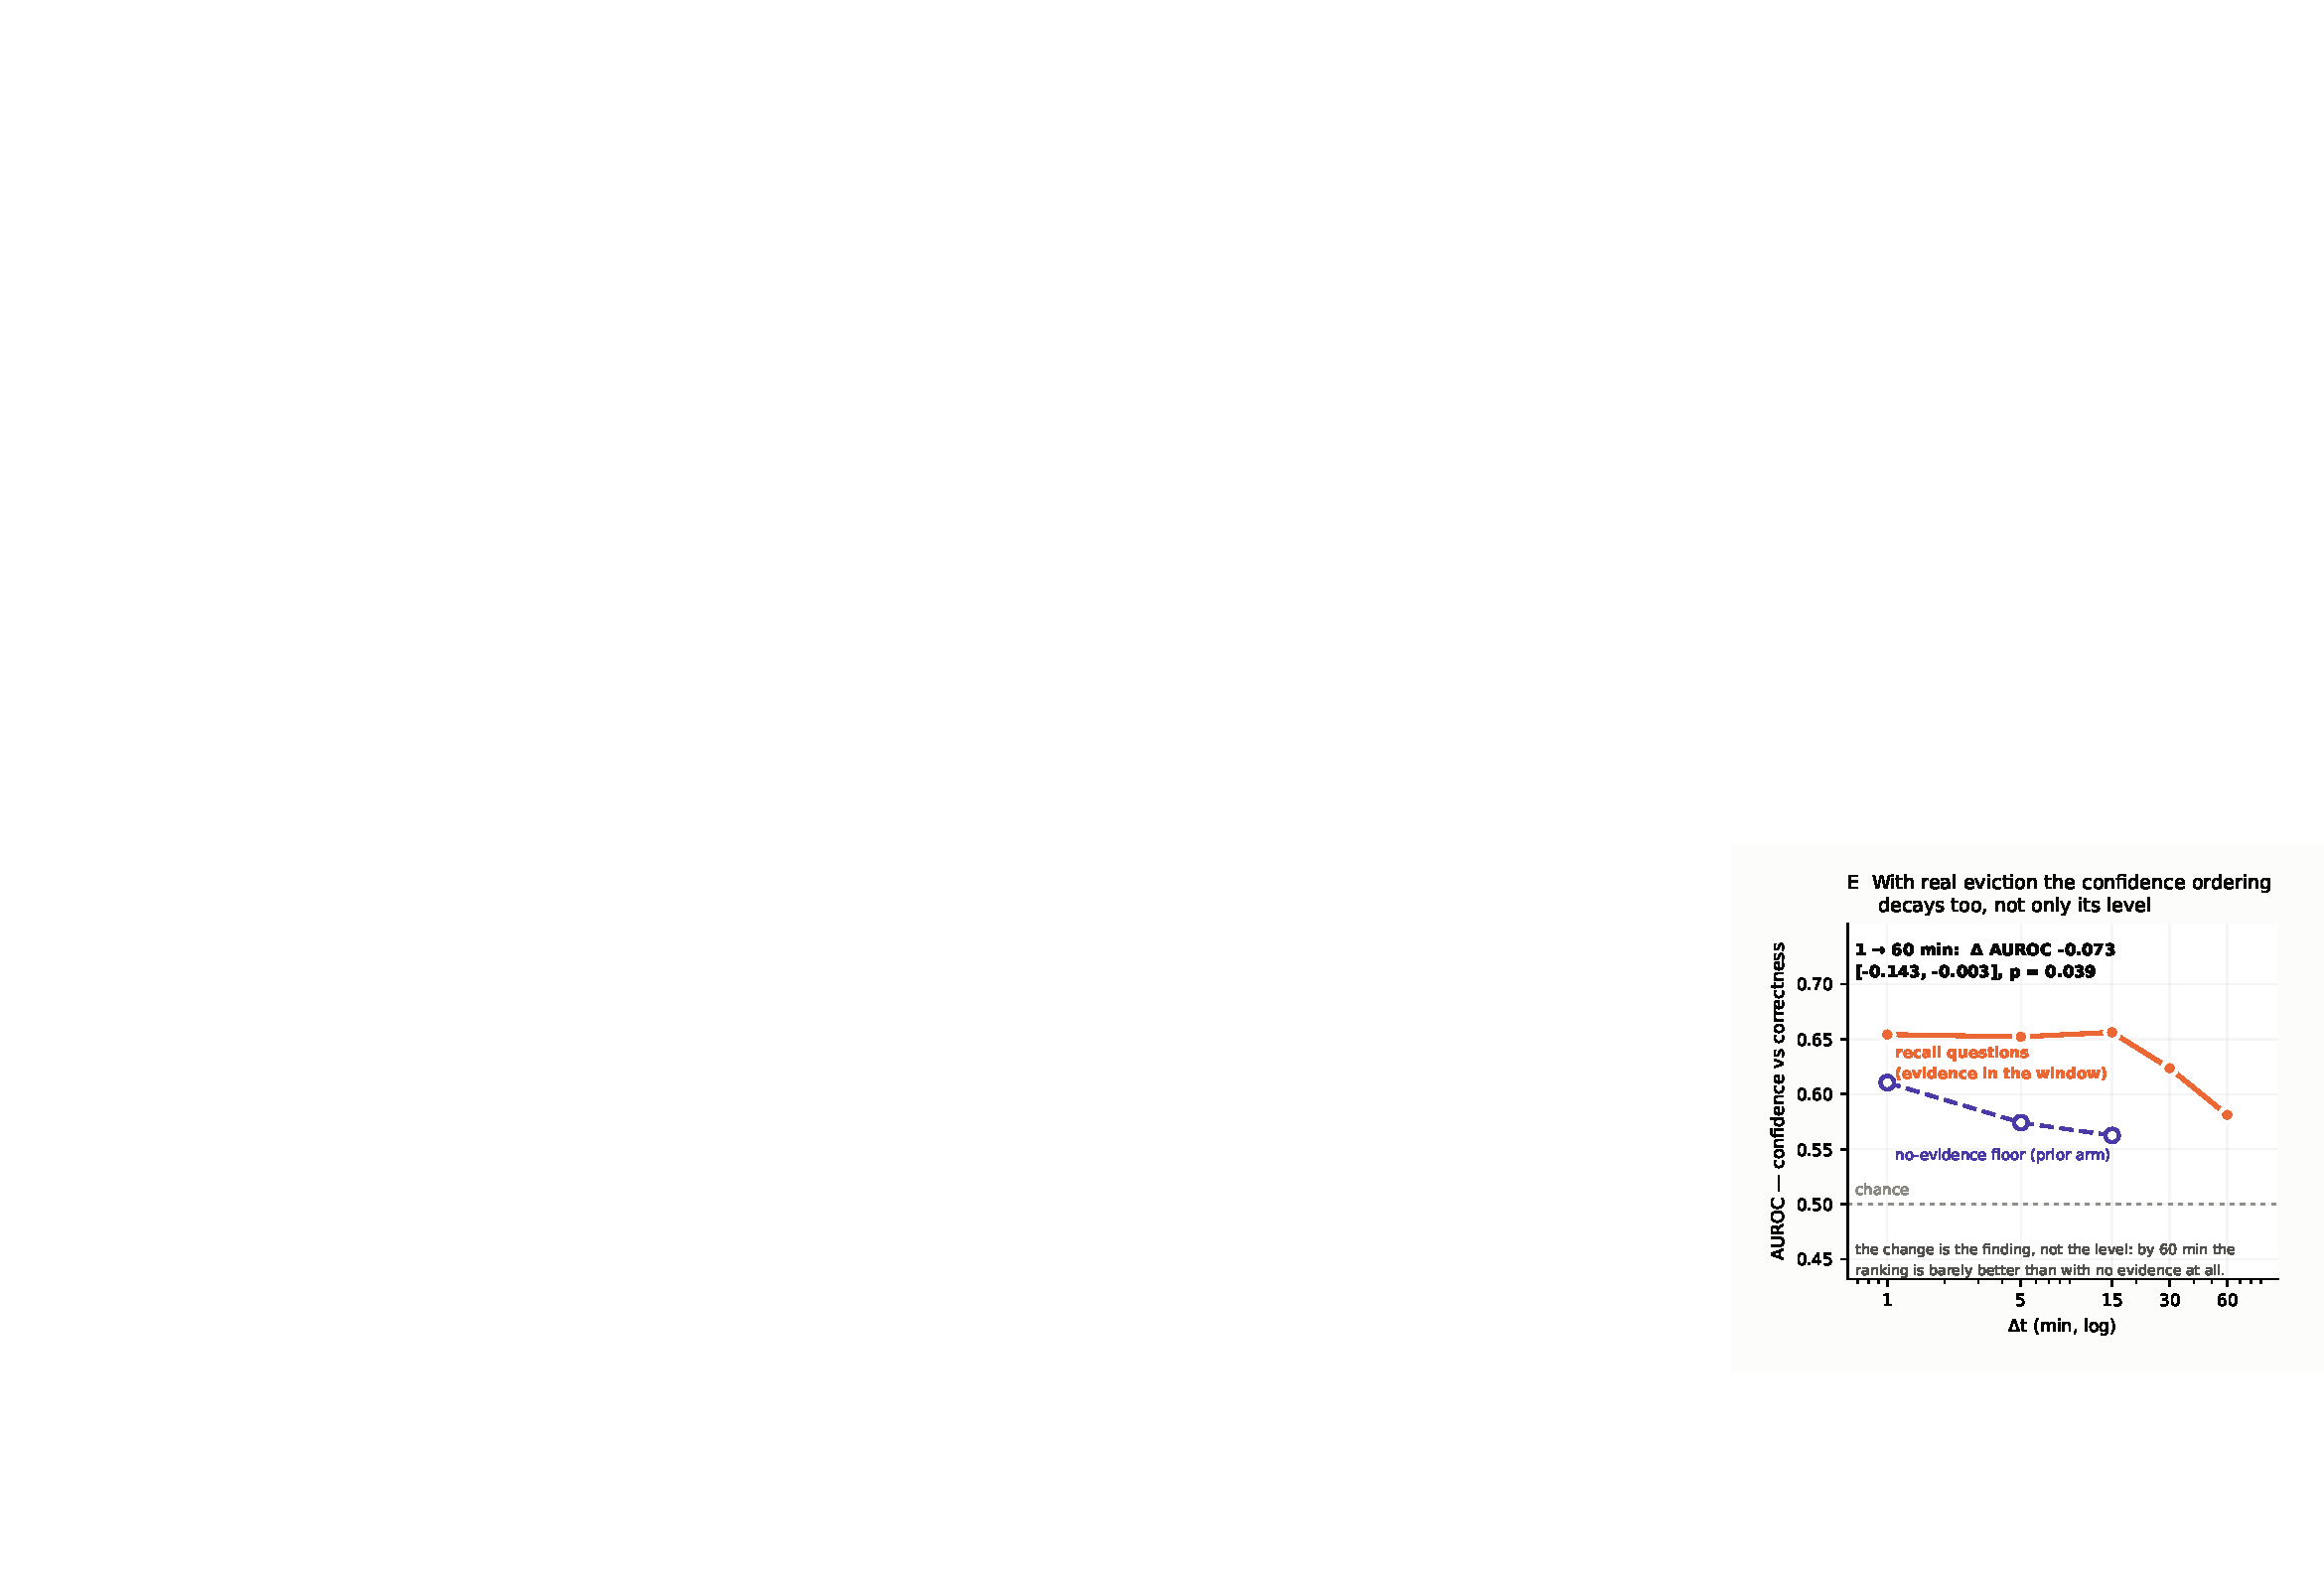
\includegraphics[width=\textwidth,height=0.55\textheight,keepaspectratio]{e2-e.pdf}
      \vskip0.1em
      {\scriptsize\color{inkmid}AUROC of confidence against correctness over the \dt\ sweep.}
    \end{column}
    \begin{column}{0.54\textwidth}
      {\scriptsize\textbf{AUROC} = how well confidence \emph{ranks} correct above incorrect answers (1.0 = perfect separation, 0.5 = chance). Invariant to confidence level --- a pure ranking measure.}
      \vskip0.3em
      {\footnotesize AUROC change, \dt\ 1\,$\rightarrow$\,60\,min:}
      \vskip0.2em
      \scriptsize
      \begin{tabular}{@{}lp{4.8cm}@{}}
        \toprule
        \Eone & \EoneAurocDelta \\
        \Etwo & \EtwoAurocDelta\newline $p$ = \EtwoAurocP \\
        \bottomrule
      \end{tabular}
      \vskip0.3em
      {\footnotesize Under full-reprocess, evidence is diluted but never removed --- the ranking stays flat. Under a bounded cache, evidence is \emph{genuinely evicted} --- and the ranking decays with it.}
    \end{column}
  \end{columns}
  \vskip0.2em
  \claim{\scriptsize Per-question confidence is a poor proxy for metamemory (P2--P3). But population-level AUROC \emph{is} sensitive to the model's memory state --- it degrades exactly when evidence is evicted. It may serve as an evaluation metric for metamemory even when the raw score does not.}
  \source{\texttt{artifacts/x9\_streaming.md}, discrimination section.}
\end{frame}
